\documentclass[../report.tex]{subfiles}
\begin{document}
\graphicspath{{img/}{../img/}}


Since all but one of the service operations on \textit{ShareIt} are private to \textit{Client}s, and some of these to \textit{User}s, it is important to discuss how access control is handled.

Two consecutive walls will block ones way when reaching \textit{ShareIt}; first a client token validation and secondly a user credential validation. \\


\begin{figure}[H]
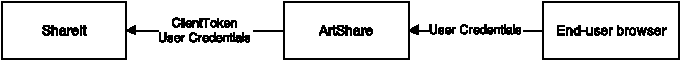
\includegraphics[width=\linewidth]{./AccessControlDeployment.pdf}
\caption{Validations in \textit{The System}}
\label{fig:validations}
\end{figure}


\subsection{Token validation}
\label{sec:Token}

The token validation is implemented as a means for \textit{ShareIt} to only allow recognized \textit{Client}s to invoke operations. This works because \textit{ShareIt} and a \textit{Client} like \textit{ArtShare} share an identical string which is called the clientToken. \textit{ShareIt}'s database has a \textit{Client} table against which \textit{ShareIt} checks incoming clientTokens. These tokens are static and do not depend on any communication session, but are created specifically for an authorized \textit{Client}, such as \textit{ArtShare}, to use.

In order to associate a token with a \textit{Client} the token has to be transferred through an encrypted channel. However security is not in scope here, which has the consequence that anybody could sniff the token.

%Below is the token which \textit{ShareIt} associates with \textit{ArtShare}. The token could be anything digital as long as its length complicates a brute force attack.

%\begin{center}
%\texttt{7dac496c534911c0ef47bce1de772502b0d6a6c60b1dbd73c1d3f285f36a0f61}
%\end{center}



\subsection{User credential validation}
\label{sec:UserCredential}

Operations on \textit{ShareIt} that need to distinguish a \textit{User} in any way take a \textit{UserDTO}. In these cases the UserDTO is validated with the database on its username and password properties. An example is the operation to validate whether a \textit{User} is registered with \textit{The System}. The clientToken argument discussed in section \ref{sec:Token} can also be seen here. 

\begin{center}
\begin{lstlisting}
	int ValidateUser(UserDTO user, string clientToken);
\end{lstlisting}
\end{center}


While the clientToken has a single purpose, namely to validate \textit{Client}s, the \textit{User} credential check is multi-functional in the way it determines many types of access rights with \textit{The System}.


\subsection{Access rights}


Access rights are used to determine a \textit{User}'s relation to \textit{Media Item}s and \textit{Client}s. This is done to ensure that no \textit{User} is granted access to operations which he does not have permission to perform. The different types of access rights and their permissions can be seen in figure~\ref{fig:accessrightmatrix}. 

\begin{figure}[H]
\centering 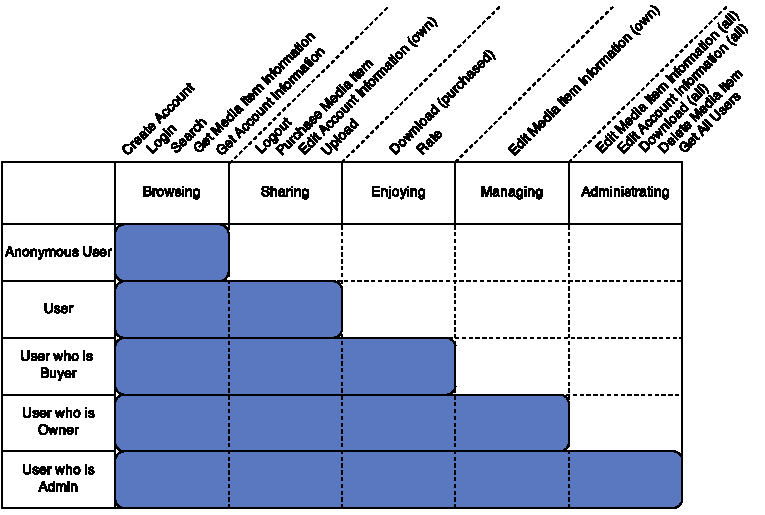
\includegraphics{AccessRightMatrix.pdf}
\caption{Access right matrix for ShareIt}
\label{fig:accessrightmatrix}
\end{figure}

Every call to a service that requires a \textit{User} will therefore validate the \textit{User}s credentials in order to determine whether they are accepted by \textit{ShareIt} (as discussed in section~\ref{sec:UserCredential}) and if the requesting \textit{User} has the correct type of access right. The method responsible for checking the access right takes both the id of the \textit{User} and the id of the \textit{Media Item} as parameters. The return type is the enum \texttt{AccessRightType} and the method has the following signature:

\begin{lstlisting}
   AccessRightType CheckUserAccess(int userId, int mediaItemId);
\end{lstlisting}


If the user credentials are not accepted an \texttt{InvalidUserException} is thrown, while an \texttt{Unauthorized- UserException} is thrown if the \textit{User} did not have the correct type of access right. 

\end{document}